\documentclass{article}

\usepackage{graphicx}
\usepackage{fancyhdr}
\usepackage[sorting=none]{biblatex}
\usepackage[margin=1in]{geometry}
\usepackage{listings}
\usepackage[hidelinks]{hyperref}
\usepackage{xcolor}
\usepackage{xepersian}

\addbibresource{bibliography.bib}
\settextfont[Scale=1]{B-NAZANIN.TTF}
\setlatintextfont[Scale=1]{Times New Roman}
\renewcommand{\baselinestretch}{1.5}
\pagestyle{fancy}
\fancyhf{}
\rhead{تکلیف اوّل امتیازی}
\lhead{\thepage}
% \rfoot{مجید فرهادی}
% \lfoot{9700000}
\renewcommand{\headrulewidth}{1pt}
\renewcommand{\footrulewidth}{1pt}

\begin{document}
\begin{titlepage}
\begin{center}

\includegraphics[width=0.3\textwidth]{./figures/sbu-logo.svg.png}\\
        
\LARGE
\textbf{دانشگاه شهید بهشتی}\\
\textbf{دانشکده مهندسی و علوم کامپیوتر}\\
        
\vfill
        
\huge
\textbf{عنوان: تکلیف اوّل امتیازی}\\
        
\vfill
        
\LARGE
% \textbf{نام و نام خانوادگی: مجید فرهادی}\\
% \textbf{شماره دانشجویی: 9700000}\\
\textbf{مدرّس: دکتر فرشاد صفایی}\\
% \textbf{طراحی : کامیاب عابدی - هادی مرادی}\\
\textbf{زمستان ۱۴۰۱}\\
\end{center}
\end{titlepage}


% \tableofcontents
\newpage
\section{پایتون مقدماتی}
\subsection{مقدمه}
زبان برنامه نویسی پایتون \lr{(Python Programming Language)}، زبانی با یادگیری آسان محسوب می‌شود. \\زیرا پایتون به عنوان یک زبان همه‌منظوره \lr{(General-Purpose Language)} ساخته و توسعه داده شده و محدود به توسعه نوع خاصی از نرم‌افزارها نیست. به بیان دیگر، می‌توان از آن برای هر کاری، از تحلیل داده\lr{(Data Analysis)}  گرفته تا ساخت بازی‌های کامپیوتری استفاده کرد. بنابراین، یادگیری پایتون بسیار حائز اهمیت است.

\subsection{بخش اوّل}
در این بخش از شما خواسته شده که با مراجعه به سایت \lr{Kaggle} دوره مربوط به آموزش پایتون را بگذرانید و \lr{certificate} مربوطه را دریافت کنید.\\

\begin{figure}[ht]
    \centering
    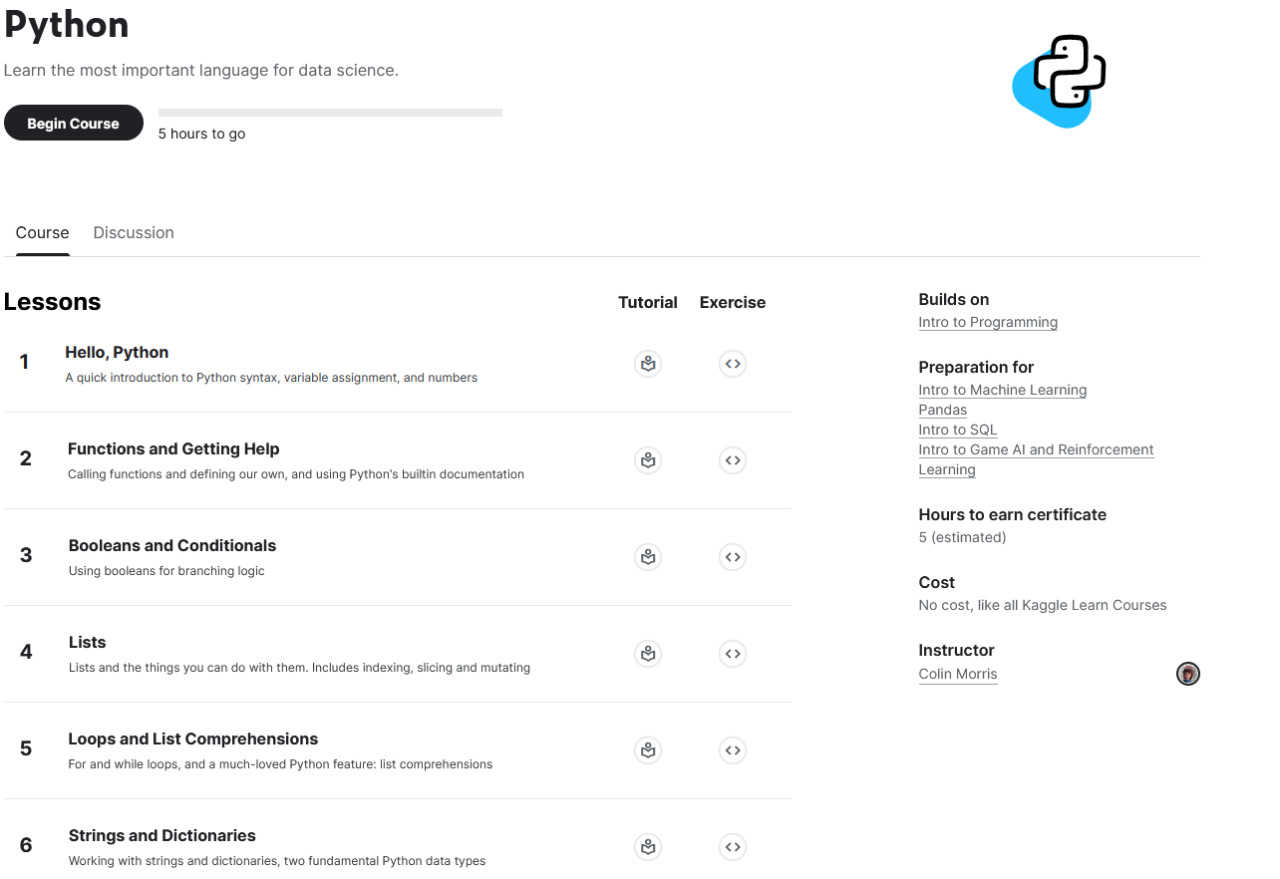
\includegraphics[width=0.8\textwidth]{./figures/kaggle_python.jpeg}
    \caption{دوره آموزش پایتون}
    \label{fig:fig1}
\end{figure}

\newpage
\subsection{بخش دوم}
در این بخش از شما خواسته شده تا لینک پروژه‌ای که در آن\lr{Certificate} و نوتبوک‌های مربوط به بخش \lr{Exercise}   قرار دارد و اسم و فامیلتان را به یک ریپوزیتوری اضافه کنید.
بنابراین لازم است شما مراحل زیر را طی کنید:
\begin{enumerate}
    \item ریپوزیتوری درس را که در پیوست لینک آن قرار داده شده است را فورک کنید.
    \item ریپوی فورک‌شده را در سیستم خود کلون کنید و اطلاعات زیر را به فایل \lr{readme} آن (همه در یک خط) اضافه کنید.\\
    نام و نام خانوادگی‌تان - لینک به پروژه‌ای که در گیتهاب قرار دادید.
    برای اینکار طبق قاعده (مثال زیر) عمل کنید.
    \lr{\lstinputlisting[language=markdown, showstringspaces=false, basicstyle=\ttfamily, backgroundcolor=\color{gray!20!white}, breaklines=true]{README.md}}
    \item کامیت‌(ها) را پوش کنید.
    \item درخواست \lr{Pull Request} دهید.    
\end{enumerate}

\section{نکته‌ها}
\begin{enumerate}
    \item نمره شما از روی پول‌ریکوئست‌های صحیح تعیین می‌شود و ربطی به مرج شدن ندارد.
    \item تا پایان مهلت تمرین فرصت دارید پول ریکوئست‌هایتان را بزنید.
    \item در صورتی که فقط می‌خواهید قسمت یک را انجام دهید (که منجر به کسر بخشی از نمره خواهد شد) اطلاعات گفته شده (نام و نام خانوادگی و لینک پروژه در گیتهاب) را در قالب یک فایل \lr{txt} زیپ‌شده به آدرس ‌‌‌‌\lr{kamyababedi@gmail.com} ایمیل کنید.
\end{enumerate}

% \section{عنوان سوال اول}
% اگر سوال بخش‌بندی‌شده نباشد، پاسخ آن در این قسمت نوشته می‌شود.
% \subsection{عنوان بخش اول سوال اول}
% پاسخ بخش اول سوال در این قسمت نوشته می‌شود.
% \subsection{عنوان بخش دوم سوال اول}
% پاسخ بخش دوم سوال در این قسمت نوشته می‌شود.

% \section{عنوان سوال دوم}
% در این قسمت با نحوه نوشتن متون دارای کلمات انگلیسی آشنا می‌شوید:\\
% \indent
% تکالیف درس سیستم‌عامل می‌بایست در قالب \lr{\LaTeX} تحویل داده شوند.

% \section{عنوان سوال سوم}
% در این قسمت با نحوه درج روابط و فرمول‌ها آشنا می‌شوید:
% \begin{center}
% $E = m{c}^{2}$
% \end{center}

% \section{عنوان سوال چهارم}
% در این قسمت با نحوه درج اشکال آشنا می‌شوید:
% \begin{figure}[ht]
%     \centering
%     \includegraphics[width=0.4\textwidth]{Sbu-logo.svg.png}
%     \caption{شکل شماره 1}
%     \label{fig:fig1}
% \end{figure}

% \section{عنوان سوال پنجم}
% در این قسمت با نحوه درج جداول آشنا می‌شوید:
% \begin{table}[ht]
%     \centering
%     \begin{tabular}{|c|c|c|}
%     \hline
%     خانه شماره 1 & خانه شماره 2 & خانه شماره 3\\
%     \hline
%     خانه شماره 4 & خانه شماره 5 & خانه شماره 6\\
%     \hline
%     خانه شماره 7 & خانه شماره 8 & خانه شماره 9\\
%     \hline
%     \end{tabular}
%     \caption{جدول شماره 1}
%     \label{tab:tab1}
% \end{table}

% \section{عنوان سوال ششم}
% در این قسمت با نحوه درج انواع لیست‌ها آشنا می‌شوید:
% \subsection{عنوان بخش اول سوال ششم}
% \begin{itemize}
%     \item [$\bullet$] مورد اول
%     \item [$\bullet$] مورد دوم
% \end{itemize}
% \subsection{عنوان بخش دوم سوال ششم}
% \begin{enumerate}
%     \item مورد شماره 1
%     \item مورد شماره 2
% \end{enumerate}

% \section{عنوان سوال هفتم}
% در این قسمت با نحوه درج برنامه‌ها آشنا می‌شوید:
% \lr{\lstinputlisting[language=C, showstringspaces=false, basicstyle=\ttfamily, backgroundcolor=\color{gray!20!white}, breaklines=true]{Source.c}}

% \section{عنوان سوال هشتم}
% در این قسمت با نحوه ارجاع به سایر منابع آشنا می‌شوید:\\
% \indent
% به صفحه درس سیستم عامل دکتر محمّدرضا حیدرپور ارجاع داده می‌شود \lr{\cite{b1}}.

% \section{ضمیمه}
% برای آشنایی بیشتر با \lr{\LaTeX}، با جست‌و‌جو در اینترنت منابع مفیدی خواهید یافت.

% %\printbibliography[title=منابع]

% \section*{منابع}
% \renewcommand{\section}[2]{}%
\begin{thebibliography}{99} % assumes less than 100 references
%چنانچه مرجع فارسی نیز داشته باشید باید دستور فوق را فعال کنید و مراجع فارسی خود را بعد از این دستور وارد کنید


\begin{LTRitems}

\resetlatinfont

\bibitem{b1} https://www.kaggle.com/learn/python
\bibitem{b1} https://github.com/SBU-CE/CE079-Graph-Theory

\end{LTRitems}

\end{thebibliography}


\end{document}
